\chapter{插图}
\label{sec:graphics}

\begin{quotation}
A picture says more than a thousand words.
\begin{flushright}
--- Shakespeare
\end{flushright}
\end{quotation}

当年~Knuth~开发~\TeX~时,GIF、JPEG、PNG、EPS~等图形格式还没有问世,所以~DVI~不能直接支持这些格式。但是高手就是高手,Knuth~在~\TeX~上留了一个后门:\verb|\special|~命令,让后面的~Driver~决定怎样处理图形。

这和当年老毛把港澳台,老邓把钓鱼岛都“留给后人解决”有异曲同工之妙。曾经有位出版社的编辑看上了包老师写的一个程序,要包老师改改当作教学辅助软件出版,但是包老师手头没有~DOS~中断的资料没办法加鼠标操作。该编辑说:你把鼠标驱动打包在软件里,让用户自己琢磨是怎么回事。

下面我们会在~\ref{sec:graphics_format}~节介绍一下~\LaTeX~所用图形格式,\ref{sec:includegraphics}~节介绍怎样插入已有的图形,\ref{sec:mp}--\ref{sec:pgf}~节讨论怎样制作矢量图形。

\section{图形格式}
\label{sec:graphics_format}

\LaTeX~支持点阵图形格式~JPEG~和~PNG,也支持矢量格式~EPS~和~PDF。对于示意图,我们应该首选矢量格式;包含大量自然色彩的图像(比如照片)应该选~JPEG,人工点阵图像应该选~PNG。

\subsection{EPS}
80~年代中后期,PS~风头之劲一时无两,人们自然会考虑把它作为文档中嵌入图形的标准格式。然而~PS~实在太强大,人们担心嵌入文档的~PS~会搞破坏,于是就产生了戴着手铐的~Encapsulated PostScript(EPS)。出于同样的原因,人们也担心嵌入~HTML~的~ActiveX、Java Applet、JavaScript~中混入恶意代码,所以才会对它们也有所限制。

早年间~DVI~经常被转换为~PS,所以~EPS~就成了~\LaTeX~的标准图形格式。

\subsection{Driver~们的口味}

\subsubsection{dvips}
\verb|dvips|~喜欢~PS,所以就爱屋及乌只支持嵌入~EPS。MiKTeX~看不惯这种垄断行为,就把~\verb|dvips|~破解,添加了对~JPEG~和~PNG~的支持。如果你反对这种黑客破解行径,只好找软件把其它图形格式转换为~EPS。

\subsubsection{pdf\LaTeX}
pdf\LaTeX~支持~JPEG、PNG和PDF,不支持~EPS。传说pdf\LaTeX~不支持~EPS~的原因是~PS~解释器的版权问题。包老师认为这种说法不可信,因为~1997~年~Hàn The Thành~发布~pdf\TeX~时~PS~已经被~PDF~赶超,Adobe~与其保护~PS~还不如保护~PDF。

\LaTeX~有两个宏包~\verb|epstopdf|~和~\verb|pst-pdf|~可以实时地(on the fly)把~EPS~转换为~PDF\footnote{在这里on the fly是指在后台处理,用户不用操心。包老师不确定把它翻译为“实时”是否合适,因为~real time~通常被翻译为实时。对于用户无须干涉、知情的情况,有人说~user transparent,也有人说~black box,语言还真奇妙。}。然而前者有安全漏洞,后者用法繁琐,用户最好还是用其它软件事先把~EPS~转为~PDF。

\subsubsection{dvipdfm}
\verb|dvipdfm|~支持~JPEG、PNG、PDF,不支持~EPS,但是它可以实时地调用~Ghostscript~把~EPS~转为~PDF。所以从图形格式支持的角度来讲,\verb|dvipdfm|~比~\verb|dvips|~和~pdf\LaTeX~都好。

那位同学说了,你这么多废话作甚,直接告诉我们用~\verb|dvipdfm|~不就完了。然而你别忘了~\verb|dvipdfm|~需要~DVI~作为输入,不幸的是用来生成~DVI~的~\verb|latex|~对~JPEG~和~PNG~有意见。

综上所述,这些~driver~都不能把图形格式痛快地通吃,所以同学们别着急,且听包老师慢慢忽悠怎样转换和处理图形格式。

\subsection{图形格式转换}

注意把点阵图形转换为矢量图形并不能提高图形本身的质量,正所谓“garbage in, garbage out”。

\subsubsection{JPEG~和~PNG~的范围框}

作为中间格式的~DVI~不包含图形本身,它只记录图形的尺寸和文件名,因为具体的图形处理由后面的~driver~负责。DVI~中图形的尺寸来自它的范围框(bounding box),而~\verb|latex|~无法从点阵图形文件中提取这一信息,所以我们需要以某种方式把范围框信息告诉它。

一种方法是打开图形文件,记下尺寸,插入图形时加上相应的参数。

另一种方法用~\verb|ebb|~程序生成一个含范围框信息的文件。比如下例会生成~\verb|graph.bb|~文件,有了它插入图形时就不需要范围框参数。注意有时此程序算出的范围框不准,不知道是它的~bug~还是包老师的人品问题。
\begin{code}
ebb graph.jpg
\end{code}

\subsubsection{其它格式转为EPS}
有很多程序都可以把点阵图形转换为~EPS,比如~\href{http://www.imagemagick.org/}{ImageMagick},以及~\href{http://www.tex.ac.uk/cgi-bin/texfaq2html?label=dvipsgraphics}{~a2ping/sam2p、bmeps、jpeg2ps、sam2p}~等。

PS~从~Level 2~开始才支持点阵图形压缩,所以在把其它格式转为~EPS~时应尽量使用~Level 2~或~3,否则输出的~EPS~会很大。

下面是一个~ImageMagick~中~\verb|convert|~程序的例子。
\begin{code}
convert photo.jpg eps2:photo.eps
\end{code}

另外还有一种~PS~虚拟打印机的方法,优点是可以把几乎所有文件“打印”成~EPS,缺点是输出的是~PS Level 1,即使驱动程序提供了其它~Level~的选项。

\begin{enumerate}
\item 找一个~PS~打印机驱动程序。Windows~安装盘附带很多打印机驱动,其中带~PS~字样的就是~PS~驱动。包老师选的是“HP Color LaserJet 8550-PS”,Adobe~提供的~PS~驱动效果不太好。其它驱动安装过程可能稍有不同。
\item 安装时端口选“FILE”,或者后面打印时选择“Print to File”。高级选项里的~PS~选项选“Encapsulated PostScript (EPS)”。
\item 打开点阵图形文件,打印到上面的虚拟打印机,输出的文件就是~EPS,但是它没有范围框。
\item 用~GSview~打开上面生成的~EPS,不用理会没范围框的警告,Options~菜单里选上“EPS Clip”,用~File~菜单的“PS to EPS”生成含范围框的~EPS。
\end{enumerate}

\subsubsection{其它格式转为~PDF}

\LaTeX~附带的~\verb|epstopdf|~程序\footnote{这个命令行程序和上面提到的~epstopdf~宏包是两样东西。}可以把~EPS~转为~PDF。类似地我们也可以安装一个~PDF~虚拟打印机,用它来把其它图形文件转为~PDF。

\section{插入图形}
\label{sec:includegraphics}

\subsection{插入命令}
如今万事俱备,只欠插入。上回讲到哪儿来着?Yeah,~Knuth~的后门~\verb|\special|。

用低级命令~\verb|\special|~来插入图形很不爽,于是~\LaTeX~v2.09~增加了~\verb|epsf|~和~\verb|psfig|~宏包。之后~\LaTeXe~推出了更好的~\verb|graphics|~和~\verb|graphicx|~宏包,这两个宏包有个共同的命令:\verb|\includegraphics|。\verb|graphicx|~版本的语法更简单,功能更强大,所以一般推荐用它。

插入图形的具体命令如下,如果是点阵图形需要加范围框参数(左上角和右下角坐标)。

\begin{code}
\includegraphics[bb=0 0 410 307]{photo.jpg}
\end{code}

若想省略文件后缀,可在插入图形前使用两个命令。前者指定一个后缀列表,让~\LaTeX~自行查找;后者告诉~\LaTeX~未知后缀的都是~EPS。
\begin{code}
\DeclareGraphicsExtensions{.eps,.mps,.pdf,.jpg,.png}
\DeclareGraphicsRule{*}{eps}{*}{}
\end{code}

\subsection{缩放、旋转}
\Fref{tab:scale_angle}~和\Fref{tab:clip}~的选项可以用来缩放、旋转和裁剪插图。

\begin{table}[htbp]
\caption{includegraphics~命令的缩放和旋转选项}
\label{tab:scale_angle}
\centering
\begin{tabularx}{350pt}{lX}
    \toprule
    scale & 缩放比例 \\
    width & 宽度 \\
    height & 高度 \\
    totalheight & 范围框高度,旋转时它不等于高度 \\
    keepaspectratio & 如果不使用它而同时指定插图的宽度、高度,长宽比可能会失调;使用它时长宽比不变,宽度、高度都不超过指定参数 \\
    angle & 旋转角度 \\
    origin & 旋转原点 \\
    \bottomrule
\end{tabularx}
\end{table}

\begin{table}[htbp]
\caption{includegraphics~命令的裁剪选项}
\label{tab:clip}
\centering
\begin{tabularx}{350pt}{lX}
    \toprule
    viewport & 可视区域的左上角和右下角坐标。\\
    trim & 左、下、右、上四边裁剪的数值。\\
    clip & 是否真正裁剪。缺省为false,不执行裁剪,多出的部分就那样放着;设置为true时执行裁剪。似乎是多此一举。\\
    \bottomrule
\end{tabularx}
\end{table}

若想深入了解~\LaTeX~插入图形的功能,请参考~Keith Reckdahl~的《Using Imported Graphics in \LaTeX~ and pdf\LaTeX》\citep{Reckdahl_2006}(简称epslatex)。

\subsection{figure环境}
插图通常需要占据大块空白,所以在文字处理软件中用户经常需要调整插图的位置。\LaTeX~有一个~\verb|figure|~环境可以自动完成这样的任务,这种自动调整位置的环境称作浮动环境。

\begin{code}
\begin{figure}[htbp]%位置选项
\centering
\includegraphics[bb=0 0 410 307,scale=.8]{photo}
\caption{10个月大的Anna}
\label{fig:anna}
\end{figure}
\end{code}

\begin{figure}[htbp]
\centering
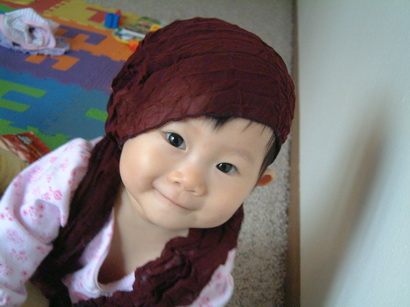
\includegraphics[bb=0 0 410 307,scale=.8]{dscf4684}
\caption{10个月大的Anna}
\label{fig:anna}
\end{figure}

上述代码中,\verb|[htbp]|~选项用来指定插图排版的理想位置,这几个字母分别代表~here、top、bottom、float page,也就是固定位置、页顶、页尾、单独的浮动页。我们可以使用这几个字母的任意组合,一般不推荐单独使用~\verb|[h]|,因为那个位置也许很不合适,\LaTeX~会很生气。

\verb|\centering|~用来使插图居中,\verb|\caption|~命令设置插图标题,\LaTeX~会自动给浮动环境的标题加上编号。注意~\verb|label|~应放在\verb|caption|~之后,否则引用时指向的是前一个插图。

\subsection{插入多幅图形}
\subsubsection{并排摆放,共享标题}
当我们需要两幅图片并排摆放,并共享标题时,可以在~\verb|figure|~环境中使用两个~\verb|\includegraphics|~命令。

\begin{fdemo}{
\centering
\includegraphics[scale=2]{examples/subfig_left.mps}
\includegraphics[scale=2]{examples/subfig_right.mps}
\captionof{figure}{反清复明}
}
\begin{figure}[htbp]
\centering
\includegraphics{left}
\includegraphics{right}
\caption{反清复明}
\end{figure}
\end{fdemo}

\subsubsection{并排摆放,各有标题}
如果想要两幅并排的图片各有自己的标题,可以在~\verb|figure|~环境中使用两个~\verb|minipage|~环境,每个环境里插入一个图。
\begin{code}
\begin{figure}[htbp]
\centering
\begin{minipage}[t]{0.3\textwidth}
    \centering
    \includegraphics{left}
    \caption{清明}
\end{minipage}
\end{code}
\begin{code}
\begin{minipage}[t]{0.3\textwidth}
    \centering
    \includegraphics{right}
    \caption{反复}
\end{minipage}
\end{figure}
\end{code}

\begin{figure}[htbp]
\centering
\begin{minipage}[t]{0.3\textwidth}
    \centering
    \includegraphics[scale=2]{examples/subfig_left.mps}
    \caption{清明}
\end{minipage}
\begin{minipage}[t]{0.3\textwidth}
    \centering
    \includegraphics[scale=2]{examples/subfig_right.mps}
    \caption{反复}
\end{minipage}
\end{figure}

\subsubsection{并排摆放,共享标题,各有子标题}
如果想要两幅并排的图片共享一个标题,并各有自己的子标题,可以使用~\verb|subfig|~宏包提供的~\verb|\subfloat|~命令。

\verb|subfloat|~命令缺少宽度参数。虽然我们可以用~\verb|\hspace|~命令调整子图的距离,子标题却只能和子图本身一样宽,就会出现折行。
\begin{code}
\usepackage{subfig}
\begin{figure}[htbp]
\centering
\subfloat[清明]{
    \label{fig:subfig_a}
    \includegraphics{left}
}
\hspace{80pt}
\subfloat[反复]{
    \label{fig:subfig_b}
    \includegraphics{right}
}
\caption{反清复明}
\end{figure}
\end{code}

每个子图可以有各自的引用,就象这个样子:\Fref{fig:subfig_a}、\Fref{fig:subfig_b}。
\begin{figure}[htbp]
\centering
\subfloat[清明]{
    \label{fig:subfig_a}
    \includegraphics[scale=2]{examples/subfig_left.mps}
}
\hspace{80pt}
\subfloat[反复]{
    \label{fig:subfig_b}
    \includegraphics[scale=2]{examples/subfig_right.mps}
}
\caption{反清复明}
\end{figure}

\subsubsection{改进的子图方法}
为了避免子标题折行,我们可以在~\verb|\subfloat|~里再嵌套个~\verb|minipage|,因为后者是有宽度的。
\begin{code}
\begin{figure}[htbp]
\centering
\subfloat[清明]{
\label{fig:improved_subfig_a}
\begin{minipage}[t]{0.3\textwidth}
    \centering
    \includegraphics{left}
\end{minipage}
}
\subfloat[反复]{
\label{fig:improved_subfig_b}
\begin{minipage}[t]{0.3\textwidth}
    \centering
    \includegraphics{right}
\end{minipage}
}
\caption{反清复明}
\end{figure}
\end{code}

\begin{figure}[htbp]
\centering
\subfloat[清明]{
\begin{minipage}[t]{0.3\textwidth}
    \centering
    \includegraphics[scale=2]{examples/subfig_left.mps}
\end{minipage}
}
\subfloat[反复]{
\begin{minipage}[t]{0.3\textwidth}
    \centering
    \includegraphics[scale=2]{examples/subfig_right.mps}
\end{minipage}
}
\caption{反清复明}
\end{figure}

\section{图形绘制工具比较}
与~\LaTeX~配套使用的绘图工具主要有三种:\MP、PSTricks~和~PGF,它们的特点如下。

\begin{itemize}
\item 工作方式。\MP~离线绘图,生成的~EPS~可以插入~\LaTeX~文档;PSTricks~和~PGF~都采用在线绘图的方式,也就是~\LaTeX~文档内直接使用绘图命令。
\item 兼容性。\MP~生成的~MPS~需要先转为~PDF~才能被~pdf\LaTeX~使用;PSTricks~生成的~EPS和~pdf\LaTeX~不兼容;PGF~提供针对各种~driver~的接口,兼容性最好。
\item 功能。PSTricks~有~PS~作后盾,功能最强;\MP~擅长处理数学内容;PGF~的流程图有独到之处。
\end{itemize}

限于篇幅,本文只对这三种工具进行简介。除了它们,用户也可以考虑一些面向~\LaTeX~的绘图前端,比如~Unix/Linux~下的~xfig~和~Windows~下的~TpX;或可以输出~EPS~的专用软件,比如~gnuplot~和~Matlab。

\section{\MP}
\label{sec:mp}

1989~年~John D. Hobby\footnote{Hobby 1985年从斯坦福获博士学位,导师就是Knuth,现供职于贝尔实验室。}开始设计一种绘图语言及其编译器,也就是~\MP。\MP~从~\MF~那里获得了大量灵感和源代码,学生从导师那里顺点东西自然是手到擒来。\MP~和~\MF~语法类似,\MP~的主要优点在于是它输出的是~EPS,而且支持彩色;\MF~输出的是点阵格式,不支持彩色。Knuth~声称自己画图时只用~\MP。

从~Hobby~主页上~\MP~的更新记录看,它的最后版本是~0.63,年份是~1994。目前~Taco Hoekwater\footnote{他也是LuaTeX开发者之一。}继续~\MP~的开发工作,最新版本是~1.005。

本文只对~\MP~作简单介绍,若想深入了解请参阅~Hobby~的《A User's Manual for MetaPost》\citep{Hobby_2007}。

\subsection{准备工作}
用户一般需要把~\MP~源文件(.mp)用一个命令行程序~\verb|mpost|~编译为一种特殊的~EPS,也称作~MPS,然后再把~MPS~插入~\LaTeX~源文件中使用。
\begin{figure}[htbp]
\centering
\begin{tikzpicture}
    \node[box] (mp) {.mp};
    \node[box, right=5 of mp] (mps) {.mps};
    \path (mp) edge [arrow] node[auto] {mpost} (mps);
\end{tikzpicture}
\caption{MetaPost~的编译}
\label{fig:mp}
\end{figure}

一个~\MP~源文件可以包含多个图形,一般形式如下。代码中每行语句以~\verb|;|~结尾,注释行以~\verb|%|~起始。每个图形的绘图命令包含在一对起始和结尾声明之间。文件结尾也要有一个结尾声明。
\begin{code}
beginfig(1); %图形起始
...          %绘图命令
endfig;      %图形结尾

beginfig(2);
...
endfig;
...
end;         %文件结尾
\end{code}

假如上面的源文件名字是~\verb|fig.mp|,我们可以执行以下编译命令。
\begin{code}
mpost fig(.mp)
\end{code}

编译后就会生成“fig.1、fig.2、$\cdots$”~等文件,每个文件的后缀就是相应的图形起始声明的编号。所以此编号在一个源文件中应保持唯一,否则后生成的文件就会覆盖前面的。

这样的文件名管理起来很麻烦,插入它们时也不能省略后缀,因为~\LaTeX~不能识别它们。用~\verb|\DeclareGraphicsExtensions|~来逐一声明后缀看起来很傻,自己改文件名更傻,\verb|\DeclareGraphicsRule|~也显得不够严谨。

然而~\MP~已经考虑到这个问题,为此提供了一个文件名模板命令。把下面的代码加到源文件头部,编译输出的文件名就会是“fig-01.mps、fig-02.mps、$\cdots$”。
\begin{code}
filenametemplate "%j-%2c.mps";   %加在源文件头部
\end{code}

我们也可以把这个命令加在每个图形的起始声明之前,指定个性化的输出文件名,这样可能更便于记忆。
\begin{code}
filenametemplate "flowchart.mps" %加在每个图形前面
\end{code}

MPS~可以用~GSview~查看,我们也可以用以下命令把它转为~PDF~再用~Adobe Reader~查看。

\begin{code}
epstopdf flowchart.mps
\end{code}

\subsection{基本图形对象}
为了节省空间,本节后面的示例会略去图形起始声明和结尾声明等不重要的细节。

\subsubsection{直线}

绘图命令~\verb|draw|~把几个点以直线段连接起来。\MP~中的缺省长度单位是~bp,用户也可以使用\Fref{tab:unit}~中的其它单位。我们还可以定义一个缩放系数,把坐标都转换成此系数的倍数,这样以后想缩放图形时只要改这个系数即可。

注意~\MP~中的变量赋值符号是~\verb|:=|,而~\verb|=|~用于方程式。变量在同一源文件中只须定义一次,其后的图形中都可以使用。

\begin{fdemo}{\includegraphics{examples/line.mps}}
draw (0,0)--(40,0)--(20,20)--(0,0);
u:=10pt; %缩放系数
draw (5u,0)--(9u,0)--(7u,2u)--cycle;
\end{fdemo}

几段直线或曲线可以构成一条路径(path),在路径末尾加个~\verb|cycle|~就能构成封闭路径(closed path)。上例中的两个三角形看起来都是封闭的,但是前面这个其实不是真正的封闭路径。

\subsection{点和线宽}
\verb|drawdot|~命令可以在指定坐标画一个点,为了使它醒目些我们可以换支粗一点的画笔。\MP~中的画笔缺省是直径~0.5pt~的圆形,拿它画出来的线宽就是~0.5pt。

\begin{fdemo}{\includegraphics{examples/dot.mps}}
draw (0,0)--(10u,4u);
pickup pencircle scaled 2pt;
drawdot (0,0);
drawdot (10u,4u);
\end{fdemo}

上面的~\verb|pickup|~是一种全局操作,也就是说它会影响到之后所有的绘图命令,我们也可以用~\verb|withpen|~为单个绘图命令设置画笔。

\begin{code}
draw (0,0)--(10u,4u) withpen pencircle scaled 2pt;
\end{code}

\subsubsection{曲线}
曲线和直线的命令相近,只是把连接两个点的~\verb|--|~换成了~\verb|..|。如果共用一些坐标,直线和曲线也可以混在一条语句里画。

\begin{fdemo}{\includegraphics{examples/curve.mps}}
draw (0,.5u)..(5u,3u)..(10u,1.5u)..
    (7u,0)..(5u,1.5u)..(7u,1.5u);
\end{fdemo}

\MP~的曲线用三次贝塞尔(Cubic B\'ezier)算法实现。用户可以在命令中增加~direction(方向)、Tension(张力)和~Curl(曲率)等控制,限于篇幅本文不赘述。

\subsubsection{预定义图形}
~\verb|fullcircle|~命令以原点为圆心画一个单位圆,类似的预定义图形还有~\verb|halfcircle、quartercircle、unitsquare|~等。注意单位正方形的参考点在左下而不在其中心。

通过不同的横向和纵向缩放系数,我们可以把圆形和正方形变成椭圆和长方形。

\begin{code}
draw fullcircle scaled 2u;
draw halfcircle scaled 2u shifted (3u,0);
draw quartercircle scaled 2u shifted (5u,0);
draw fullcircle xscaled 4u yscaled 2u shifted (9u,0);
draw unitsquare scaled 2u shifted (12u,-u);
draw unitsquare xscaled 4u yscaled 2u shifted (15u,-u);
\end{code}

\begin{out}
\includegraphics{examples/predefined.mps}
\end{out}

\subsection{图形控制}

\subsubsection{线型和箭头}
在绘制图形时,我们不仅可以变换线宽,也可以使用多种线型。
\begin{code}
draw (0,0)--(10u,0) dashed withdots;
draw (0,1u)--(10u,1u) dashed withdots scaled 2;
draw (0,2u)--(10u,2u) dashed evenly;
draw (0,3u)--(10u,3u) dashed evenly scaled 2;
\end{code}

\begin{out}
\includegraphics{examples/dashed.mps}
\end{out}

箭头和直线、曲线的语法相近,注意画反向箭头时需要把两个坐标用一对~\verb|()|~括起来。

\begin{fdemo}{\includegraphics{examples/arrow.mps}}
drawarrow (0,4u)--(9u,4u);
drawarrow reverse ((0,2u)--(9u,2u));
drawdblarrow (0,0)--(9u,0);
\end{fdemo}

\subsubsection{颜色和填充}
\MP~预定义的颜色有黑、白、红、绿、蓝,它们的~RGB~值分别为(0,0,0)、(1,1,1)、(1,0,0)、(0,1,0)、(0,0,1),缺省色就是黑色。

绘图命令一般都可以通过~\verb|withcolor|~参数来使用各种颜色。封闭路径可以用~\verb|fill|~命令填充。

\begin{fdemo}{\includegraphics{examples/color.mps}}
draw (0,4u)--(9u,4u) withcolor red;
draw (0,2u)--(9u,2u) withcolor green;
draw (0,0)--(9u,0) withcolor blue;
\end{fdemo}

\begin{code}
fill p scaled u;
fill p scaled u shifted (3u,0) withcolor red;
fill p scaled u shifted (6u,0) withcolor green;
fill p scaled u shifted (9u,0) withcolor blue;
\end{code}

\begin{out}
\includegraphics{examples/fill.mps}
\end{out}

另一个命令~\verb|filldraw|~可以看作是~\verb|fill+draw|,它除了填充外还会把路径用指定的画笔画一遍。然而不幸的是画边缘和填充内部只能用同一种颜色,所以它的用处不大。

除了为每个绘图命令单独指定颜色,我们也可以使用一个全局命令,使得其后的绘图命令都使用某种颜色。
\begin{code}
drawoption(withcolor blue);
\end{code}

下面的方法可以用来定义基本色以外的颜色,用基本色混色或直接用RGB值效果是一样的。

\begin{code}
color c[];
c1 := .9red + .6green + .3blue;
c2 := (.9,.6,.3);
\end{code}

\subsubsection{图形变换}
我们可以对路径进行缩放、平移、旋转等变换操作,横向和纵向缩放可以分开进行。由于旋转是围绕原点进行的,所以要注意平移和旋转的顺序。下例中定义了一个~\verb|path|~变量,以便后面重用。

\begin{code}
path p;
p := (0,0)--(2,0)--(1,1.732)--cycle;
draw p scaled u;
draw p xscaled 2u yscaled u shifted (3u,0);
draw p scaled u rotated 60 shifted (8u,0);
\end{code}

\begin{out}
\includegraphics{examples/transform.mps}
\end{out}

\subsubsection{标注}
\verb|\label|~命令可以在指定的点附近加文字标注。\MP~也可以用一对~\verb|btex|~和~\verb|etex|~来嵌入一些~\TeX~内容,比如数学标注。

\begin{code}
draw unitsquare xscaled 10u yscaled 4u;
label.top("top", (5u,4u));
label.bot("bottom", (5u,0));
label.lft("left", (0,2u));
label.rt("right", (10u,2u));
\end{code}
\begin{code}
label.ulft("upper left", (0,4u));
label.urt("upper right", (10u,4u));
label.llft("lower left", (0,0));
label.lrt("lower right", (10u,0));
label.rt(btex $E=mc^2$ etex, (3u,2u));
\end{code}

\begin{out}
\includegraphics{examples/label.mps}
\end{out}

因为用缺省方法编译生成的~MPS~不嵌入字体,当~\MP~包含文字时,GSview~就不能正常查看。这时我们可以给编译命令加个参数,生成的~MPS~就会包含字体信息。注意这种方法生成的~MPS~虽然~GSview~能查看,\verb|dvipdfmx|~却不能正常处理。

\begin{code}
mpost \prologues:=2; input fig.mp
\end{code}

\subsection{编程功能}

\subsubsection{数据类型和变量}
\MP~中有10~种基本数据类型:numeric、pair、path、pen、~color~、cmykcolor、transform、string、boolean、picture。我们已经接触过其中几种,比如缩放系数~u~就是一个~numeric,一个点的坐标是一个~pair,几个点用直线或曲线连起来是一个~path,pencircle~是一种~pen,black~是一种~color,scaled、rotated、shifted~都是~transform。

numeric~类型变量的精度是~1/65536,它的绝对值不能超过~4096,在计算过程中数值可以达到~32768。这样的规定也应归功于当年的电脑硬件,不过对于科技文档插图而言,4096~一般还是够用的。

除了缺省的~numeric,其它变量在使用之前都需要用数据类型来显式声明。相同类型的变量可以在一行语句中声明,但是带下标的变量不能放在同一行(这个规定很蹊跷)。
\begin{code}
numeric x,y,z;    %正确
numeric x1,x2,x3; %错误
numeric x[];      %正确
\end{code}

\subsubsection{数学运算}
\MP~中可以使用普通的运算符,比如~\verb|+ - * /|;也提供一些特殊的运算符,比如~\verb|a++b|~表示$\sqrt{a^2+b^2}$,\verb|a+-+b|~表示$\sqrt{a^2-b^2}$;另外\Fref{tab:math_function}~列出一些常用数学函数。

\begin{table}[htbp]
\caption{数学函数}
\label{tab:math_function}
\centering
\begin{tabular}{llll}
    \toprule
    abs     & 绝对值   & mexp & 指数 \\
    round   & 四舍五入 & mlog & 对数 \\
    ceiling & 向上圆整 & sind & 正弦 \\
    floor   & 向下圆整 & cosd & 余弦 \\
    mod     & 模余     & normaldeviate & 正态分布随机数 \\
    sqrt    & 开方     & uniformdeviate & 均匀分布随机数 \\
    \bottomrule
\end{tabular}
\end{table}

\subsubsection{循环}
当执行重复任务时,循环语句可以让程序变得简洁。注意下例中的循环语句是一条命令,之所以分成三行写是为了看起来清晰点。

\begin{fdemo}{\includegraphics{examples/loop.mps}}
draw (0,0) %注意这里没有分号
for x=1 upto 3: 
    ..(x*x,x)*u 
endfor;
\end{fdemo}

循环语句缺省步长是~1,我们也可以改用其它步长。\verb|upto|~其实就是~\verb|step 1 until|~的缩写方式。
\begin{code}
for x=1 step .5 until 3: 
\end{code}

\section{PSTricks}
\label{sec:pstricks}

PSTricks~是一个基于~PS~的宏包,有了它用户就可以直接在~\LaTeX~文档中插入绘图命令。PSTricks~早期的作者是~Timothy Van Zandt\footnote{法国Insead大学经济系教授。},初始开发年月不详,他于~1997~年退居二线,之后由~Denis Girou、Sebastian Rahtz\footnote{牛津大学计算机系网管。}、Herbert Voß~等维护。

本文只介绍~PSTricks~的基本功能,若想深入了解请参阅~Van Zandt~的《PSTricks User's Guide》\citep{Zandt_2007}。另外\Fref{tab:pst_add}~列出了一些可以和~PsTricks~配合使用的辅助宏包。

\begin{table}[htbp]
\caption{PSTricks~辅助宏包}
\label{tab:pst_add}
\centering
\begin{tabular}{llll}
    \toprule
    multido & 循环语句    & pst-eucl & 几何函数 \\    
    pst-plot & 函数绘图   & pst-math & 弧度三角函数 \\
    pst-plot3d & 三维绘图 & pstricks-add & 极坐标 \\  
    \bottomrule
\end{tabular}
\end{table}

\subsection{准备工作}
首先要引入~PSTricks~宏包。PSTricks~中缺省长度单位是~1cm,我们也可以设置自己的单位。
\psset{unit=10pt}
\begin{code}
\usepackage{pstricks}
\psset{unit=10pt}
\end{code}

绘图命令一般要放在~\verb|pspicture|~环境里,这样~\LaTeX~就会给图形预留一个矩形区域,注意这个矩形要能容纳所有图形对象。为了节省空间,在本节后面的示例代码中,~\verb|pspicture|~环境将被略去。

\begin{code}
\begin{pspicture}(0,0)(4,2)
...
\end{pspicture}
\end{code}

另外需要注意的是,嵌入~\LaTeX~的~PSTricks~生成的是~PS,\verb|dvips|~可以处理,\verb|dvipdfm|~和pdf\LaTeX~则不能。所以如果使用后两种~driver,需要先行生成~EPS。

第一种方法是把~PSTricks~代码放进一个空白的\LaTeX~页面,用它生成一个简单的~DVI。

\begin{code}
\documentclass{article}
\usepackage{pstricks}
\pagestyle{empty}   %页面样式为空

\begin{document}
\psset{unit=10pt}
\colorbox{white}{%
    \begin{pspicture}(0,0)(4,2)%
    \psdot(0,0)%
    \psdots(0,2)(2,2)(4,2)%
    \end{pspicture}%
}
\end{document}
\end{code}

然后用以下命令把~DVI~转为~EPS,\verb|-E|~参数即代表~EPS。上面代码中的~colorbox~使得生成的~EPS~有正确的范围框。

\begin{code}
dvips pst_dots(.dvi) -E -o dots.eps
\end{code}

第二种方法是用~\verb|pst-eps|~宏包,它能够在线处理~PSTricks~代码并生成~EPS,这样用户就可以在同一文件中使用该~EPS。

然而~\verb|dvipdfmx|~不能正确处理~\verb|pst-eps|~生成的~EPS。它和~\verb|\rput|、\verb|\uput|~命令,\verb|pst-plot|~宏包中的~\verb|\psaxes|~命令都不兼容。类似的~\verb|ps4pdf|~宏包和~\verb|tabularx|~宏包不兼容。

\begin{comment}
\usepackage{pst-eps}
\PSTtoEPS[bbllx=0,bblly=0,bburx=4,bbury=2,makeeps=all]
{dots.eps}{
    \psdot(0,0)
    \psdots(0,2)(2,2)(4,2)
}
\includegraphics{dots.eps}
\end{comment}

\subsection{基本图形对象}
\subsubsection{点}
我们可以用以下命令画一个或多个点。
\begin{comment}
\PSTtoEPS[bbllx=0,bblly=0,bburx=4,bbury=2,makeeps=all]
{examples/dot.eps}{
    \psdot(0,0)
    \psdots(0,2)(2,2)(4,2)
}
\end{comment}

\begin{fdemo}{
\includegraphics{examples/pst_dot.eps}}
\psdot(0,0)
\psdots(0,2)(2,2)(4,2)
\end{fdemo}

\subsubsection{直线、多边形、矩形}
\verb|\psline|~命令把多个点用直线段连接起来,线段之间的连接缺省为尖角,也可以设置圆角。
\begin{comment}
\PSTtoEPS[bbllx=0,bblly=0,bburx=9,bbury=2,makeeps=all]
{examples/line.eps}{
    \psline(0,0)(2,2)(4,0)
    \psline[linearc=.3](5,0)(7,2)(9,0)
}
\end{comment}

\begin{fdemo}{
\includegraphics{examples/pst_line.eps}}
\psline(0,0)(2,2)(4,0)
\psline[linearc=.3](5,0)(7,2)(9,0)
\end{fdemo}

\verb|\pspolygon|~命令和~\verb|\psline|~类似,但是它会形成封闭路径。
\begin{comment}
\PSTtoEPS[bbllx=0,bblly=0,bburx=9,bbury=2,makeeps=all]
{examples/polygon.eps}{
    \pspolygon(0,0)(2,2)(4,0)
    \pspolygon[linearc=.3](5,0)(7,2)(9,0)
}
\end{comment}

\begin{fdemo}{
\includegraphics{examples/pst_polygon.eps}}
\pspolygon(0,0)(2,2)(4,0)
\pspolygon[linearc=.3](5,0)(7,2)(9,0)
\end{fdemo}

矩形用~\verb|\psframe|~命令,其参数就是矩形左下角和右上角的坐标。矩形也可以设置圆角。
\begin{comment}
\PSTtoEPS[bbllx=0,bblly=0,bburx=9,bbury=2,makeeps=all]
{examples/frame.eps}{
    \psframe(0,0)(4,2)
    \psframe[framearc=.3](5,0)(9,2)
}
\end{comment}

\begin{fdemo}{
\includegraphics{examples/pst_frame.eps}}
\psframe(0,0)(4,2)
\psframe[framearc=.3](5,0)(9,2)
\end{fdemo}

\subsubsection{圆、椭圆、圆弧、扇形}
圆形用~\verb|\pscircle|~命令,参数是圆心和半径。椭圆用~\verb|\psellipse|~命令,参数是中心、长径、短径。注意这两个命令的半径参数用不同的括号,可能是作者的笔误。
\begin{comment}
\PSTtoEPS[bbllx=0,bblly=0,bburx=7,bbury=2,makeeps=all]
{examples/circle.eps}{
    \pscircle(1,1){1}
    \psellipse(5,1)(2,1)
}
\end{comment}

\begin{fdemo}{
\includegraphics{examples/pst_circle.eps}}
\pscircle(1,1){1}
\psellipse(5,1)(2,1)
\end{fdemo}

圆弧用~\verb|\psarc|~命令,其参数是圆心、半径、起止角度,逆时针作图。~\verb|\psarcn|~类似,只是顺时针作图。扇形用~\verb|\pswedge|~命令。
\begin{comment}
\PSTtoEPS[bbllx=0,bblly=0,bburx=11,bbury=2,makeeps=all]
{examples/arc.eps}{
    \psarc(1,0){2}{0}{120}
    \psarcn(5,0){2}{120}{0}
    \pswedge(9,0){2}{0}{120}
}
\end{comment}

\begin{fdemo}{
\includegraphics{examples/pst_arc.eps}}
\psarc(1,0){2}{0}{120}
\psarcn(5,0){2}{120}{0}
\pswedge(9,0){2}{0}{120}
\end{fdemo}

\subsubsection{曲线}
\verb|\pscurve|~命令把一系列点用平滑曲线连接起来;它的变形版本~\verb|\psecurve|~命令不显示曲线的两个端点;另一变形命令~\verb|\psccurve|~则把曲线封闭起来。

参数~\verb|showpoints=true|~用来显示曲线的构成点,此参数也可用于其它绘图命令。
\begin{comment}
\PSTtoEPS[bbllx=0,bblly=0,bburx=15,bbury=2,makeeps=all]
{examples/curve.eps}{
    \pscurve[showpoints=true](0,1)(1,2)(3,0)(4,2)(1,0)
    \psecurve[showpoints=true](5,1)(6,2)(8,0)(9,2)(5,0)
    \psccurve[showpoints=true](11,1)(12,2)(14,0)(15,2)(12,0)
}
\end{comment}

\begin{code}
\pscurve[showpoints=true](0,1)(1,2)(3,0)(4,2)(1,0)
\psecurve[showpoints=true](5,1)(6,2)(8,0)(9,2)(5,0)
\psccurve[showpoints=true](11,1)(12,2)(14,0)(15,2)(12,0)
\end{code}
\begin{out}

\includegraphics{examples/pst_curve.eps}
\end{out}

\verb|\psbezier|~命令输出一条贝塞尔曲线,其参数就是曲线的控制点。
\begin{comment}
\PSTtoEPS[bbllx=0,bblly=0,bburx=6,bbury=2,makeeps=all]
{examples/bezier.eps}{
    \psbezier[showpoints=true]
        (0,0)(2,2)(4,0)(6,2)
}
\end{comment}

\begin{fdemo}{
\includegraphics{examples/pst_bezier.eps}}
\psbezier[showpoints=true]
    (0,0)(2,2)(4,0)(6,2)
\end{fdemo}

抛物线用~\verb|\psparabola|~命令,它有两个参数,第一个是抛物线通过的一点,第二个是抛物线的顶点。
\begin{comment}
\PSTtoEPS[bbllx=0,bblly=0,bburx=2,bbury=2,makeeps=all]
{examples/parabola.eps}{
    \psparabola[showpoints=true]
        (2,2)(1,0)
}
\end{comment}

\begin{fdemo}{
\includegraphics{examples/pst_parabola.eps}}
\psparabola[showpoints=true]
    (2,2)(1,0)
\end{fdemo}

\subsubsection{网格和坐标}
科技制图通常会用到坐标网格。\verb|\psgrid|~命令输出一个矩形网格,它有三个参数点。网格坐标标注在通过第一个点的两条直线上,第二和第三个点是矩形的两个对角顶点。当第一个参数省略时,坐标标注在通过第一个顶点的两条矩形边上。
\begin{comment}
\psset{unit=10pt}
\PSTtoEPS[bbllx=-1,bblly=-1,bburx=8.4,bbury=2.4,makeeps=all]
{examples/grid.eps}{
    \psgrid(0,0)(-1,-1)(3,2)
    \psgrid(5,0)(8,2)
}
\end{comment}

\begin{code}
\psgrid(0,0)(-1,-1)(3,2)
\psgrid(5,0)(8,2)
\end{code}
\begin{out}
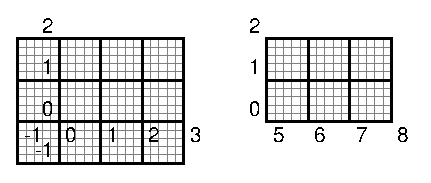
\includegraphics{examples/pst_grid.eps}
\end{out}

\verb|pst-plot|~宏包提供的~\verb|\psaxes|~命令输出坐标轴。它的参数和~\verb|\psgrid|~的类似,刻度和标注都可以灵活地设置,也可以把坐标轴改成一个矩形框的形式。
\begin{code}
\psset{unit=10pt}
\psaxes{<->}(0,0)(-1,-1)(3,2)
\psaxes[tickstyle=top,labels=none]{->}(5,0)(8,2)
\psaxes[axesstyle=frame,tickstyle=top]{->}(10,0)(13,2)
\end{code}
\begin{out}
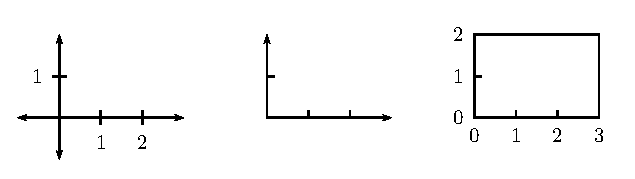
\includegraphics{examples/pst_axis.eps}
\end{out}

\subsection{图形控制}
\subsubsection{线型和箭头}
PSTricks~中的缺省线宽是~0.8pt,缺省线型是实线。以下参数可以控制单个绘图命令的线宽和线型。
\begin{comment}
\psset{unit=10pt}
\PSTtoEPS[bbllx=0,bblly=0,bburx=9,bbury=4,makeeps=all]
{examples/linestyle.eps}{
    \psline[linewidth=1.5pt](0,4)(9,4)
    \psline[linestyle=dotted](0,2)(9,2)
    \psline[linestyle=dashed](0,0)(9,0)
}
\end{comment}

\begin{fdemo}{
\includegraphics{examples/pst_linestyle.eps}}
\psline[linewidth=1.5pt](0,4)(9,4)
\psline[linestyle=dotted](0,2)(9,2)
\psline[linestyle=dashed](0,0)(9,0)
\end{fdemo}

我们也可以用命令~\verb|\psset|~命令来设置全局参数。
\begin{code}
\psset{linewidth=1pt,linestyle=dashed}
\end{code}

以下参数可以控制绘图命令的箭头。
\begin{comment}
\PSTtoEPS[bbllx=0,bblly=0,bburx=9,bbury=4,makeeps=all]
{examples/arrow.eps}{
    \psline{->}(0,4)(9,4)
    \psline{<-}(0,2)(9,2)
    \psline{<->}(0,0)(9,0)
}
\end{comment}

\begin{fdemo}{
\includegraphics{examples/pst_arrow.eps}}
\psline{->}(0,4)(9,4)
\psline{<-}(0,2)(9,2)
\psline{<->}(0,0)(9,0)
\end{fdemo}

\subsubsection{颜色和填充}
PSTricks~预定义的颜色有~black、darkgray、gray、lightgray、white~等灰度颜色,也有~red、green、blue、cyan、magenta、yellow~等彩色。我们也可以自定义灰度颜色和彩色。

\begin{code}
\newgray{mygray}{.3}
\newrgbcolor{mycolor}{.3 .4 .5}
\end{code}

以下参数可以控制单个绘图命令的颜色,我们也可以用~\verb|\psset|~命令设置全局参数。
\begin{comment}
\PSTtoEPS[bbllx=0,bblly=0,bburx=9,bbury=4,makeeps=all]
{examples/color.eps}{
    \psline[linecolor=red](0,4)(9,4)
    \psline[linecolor=green](0,2)(9,2)
    \psline[linecolor=blue](0,0)(9,0)
}
\end{comment}

\begin{fdemo}{
\includegraphics{examples/pst_color.eps}}
\psline[linecolor=red](0,4)(9,4)
\psline[linecolor=green](0,2)(9,2)
\psline[linecolor=blue](0,0)(9,0)
\end{fdemo}

以下参数可以控制单个绘图命令的填充模式和填充颜色,注意只有封闭路径才可以填充。
\begin{comment}
\PSTtoEPS[bbllx=0,bblly=0,bburx=11,bbury=2,makeeps=all]
{examples/fill.eps}{
    \pscircle[fillstyle=solid,fillcolor=red](1,1){1}
    \pscircle[fillstyle=vlines](4,1){1}
    \pscircle[fillstyle=hlines](7,1){1}
    \pscircle[fillstyle=crosshatch](10,1){1}
}
\end{comment}

\begin{code}
\pscircle[fillstyle=solid,fillcolor=red](1,1){1}
\pscircle[fillstyle=vlines](4,1){1}
\pscircle[fillstyle=hlines](7,1){1}
\pscircle[fillstyle=crosshatch](10,1){1}
\end{code}
\begin{out}
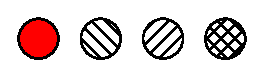
\includegraphics{examples/pst_fill.eps}
\end{out}

\subsection{对象布局}
\subsubsection{平移}
参数~\verb|origin|~可以让一个图形对象平移到指定的坐标点,我们也可以用~\verb|\psset|~命令设置全局平移参数。
\begin{comment}
\PSTtoEPS[bbllx=0,bblly=0,bburx=7,bbury=2,makeeps=all]
{examples/origin.eps}{
    \psframe(0,0)(3,2)
    \psframe[origin={4,0}](0,0)(3,2)
}
\end{comment}

\begin{fdemo}{
\includegraphics{examples/pst_origin.eps}}
\psframe(0,0)(3,2)
\psframe[origin={4,0}](0,0)(3,2)
\end{fdemo}

\subsubsection{旋转}
\verb|\rput|~命令可以对一个图形对象同时进行旋转和平移操作。它有两个参数,第一个是旋转角度,第二个是平移到的坐标点。
\begin{fdemo}{
\includegraphics{examples/pst_rput.eps}}
\psframe(0,0)(3,2)
\rput{30}(5,0){\psframe(0,0)(3,2)}
\end{fdemo}

\subsubsection{文字标注}
\verb|\rput|~命令还可以在指定的坐标点标注文字,这时它的第一个参数是坐标点相对于标注的位置。其取值可以是纵向的~t、b(上下),或横向的~l、r(左右),也可以是纵向和横向位置的组合。
\begin{fdemo}{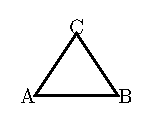
\includegraphics{examples/pst_label.eps}}
\pspolygon(0,0)(4,0)(2,3)
\rput[r](0,0){A}
\rput[l](4,0){B}
\rput[b](2,3){C}
\end{fdemo}

\verb|\rput|~生成的标注就在坐标点上,有时会感觉离图形太近。另一个命令~\verb|\uput|~则生成缺省距离指定坐标点~5pt的标注,它的第一个参数是标注相对于坐标点的角度。
\begin{fdemo}{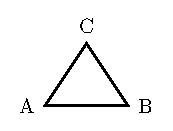
\includegraphics{examples/pst_uput.eps}}
\pspolygon(0,0)(4,0)(2,3)
\uput[l](0,0){A}
\uput[r](4,0){B}
\uput[u](2,3){C}
\end{fdemo}

\verb|\uput|~的角度参数可以是任意角度,也可以是字母,参见。注意~\verb|\uput|~的角度参数和~\verb|\rput|~命令的参考点位置参数的定义几乎正好相反,这也许反映了作者洒脱的风格。

\begin{table}[htbp]
\caption{uput~命令的角度参数}
\label{tab:uput}
\centering
\begin{tabular}{lrlr}
    \toprule
    r &   0$^\circ$ & ur &  45$^\circ$ \\
    u &  90$^\circ$ & ul & 135$^\circ$ \\
    l & 180$^\circ$ & dl & 225$^\circ$ \\
    d & 270$^\circ$ & dr & 315$^\circ$ \\
    \bottomrule
\end{tabular}
\end{table}

\section{PGF}
\label{sec:pgf}
PGF~和~Beamer~的作者都是~Till Tantau\footnote{德国Lübeck大学计算机研究所教授。}。Tantau~当初开发~Beamer~是为了应付~2003~年他的博士学位论文答辩,之后它在~CTAN~上流行开来。2005~年~PGF~从~Beamer~项目中分离出来,成为一个独立的宏包。

本文只对~PGF~作简单介绍,若想深入了解请参阅~Tantau~的《TikZ and PGF Manual》\citep{Tantau_2008}。

\subsection{准备工作}
一般人们并不直接使用~PGF~命令,而是通过它前端~TikZ~来调用~PGF。在引用~\verb|tikz|~宏包之前,用户需要设置~PGF~系统~driver。
\begin{code}
\def\pgfsysdriver{pgfsys-dvipdfmx.def}
\usepackage{tikz}
\end{code}

PGF~的缺省长度单位是~1cm,我们也可以改用其它单位。注意这样预定义的长度单位有时会失效,这可能是~PGF~的~bug。
\begin{code}
\pgfsetxvec{\pgfpoint{10pt}{0}}
\pgfsetyvec{\pgfpoint{0}{10pt}}
\end{code}

TikZ~提供一个~\verb|tikz|~命令和一个~\verb|tikzpicture|~环境,具体绘图指令可以放在~\verb|tikz|~后面,也可以放在~\verb|tikzpicture|~中间。两种方法效果相同,用户可以任意选择。为了节省空间,本节的示例将省略部分环境代码。
\begin{code}
\tikz ...   %绘图命令
\begin{tikzpicture}
...         %绘图命令
\end{tikzpicture}
\end{code}

\subsection{基本图形对象}
\subsubsection{直线、多边形、矩形}
TikZ~中直线的语法和~\MP~类似,加~\verb|cycle|~参数才能构成真正的封闭路径。
\begin{fdemo}{
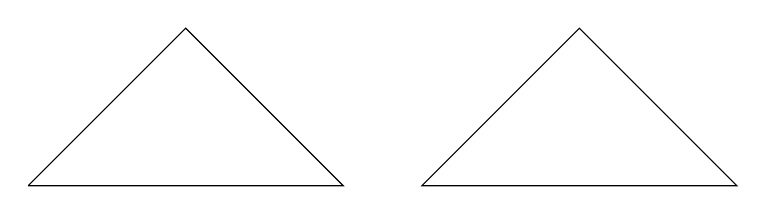
\begin{tikzpicture}
\draw (0,0)--(4,0)--(2,2)--(0,0);
\draw (5,0)--(9,0)--(7,2)--cycle;
\end{tikzpicture}
}
\draw (0,0)--(4,0)--(2,3)--(0,0);
\draw (5,0)--(9,0)--(7,3)--cycle;
\end{fdemo}

矩形命令如下,它的两个参数是矩形的两个对角顶点。
\begin{fdemo}{
\begin{tikzpicture}
\draw (0,0) rectangle (4,2);
\end{tikzpicture}
}
\draw (0,0) rectangle (4,2);
\end{fdemo}

\subsubsection{圆、椭圆、弧}
圆和椭圆命令如下,圆的参数是圆心和半径,椭圆的参数是中心、长径、短径。
\begin{fdemo}{
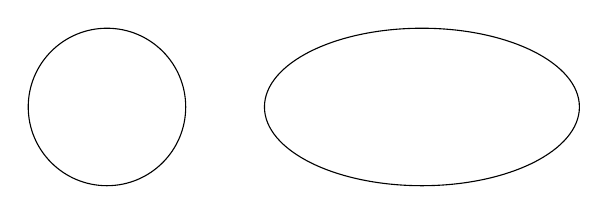
\begin{tikzpicture}
\draw (1,1) circle (1);
\draw (5,1) ellipse (2 and 1);
\end{tikzpicture}
}
\draw (1,1) circle (1);
\draw (5,1) ellipse (2 and 1);
\end{fdemo}

圆弧和椭圆弧命令如下,圆弧的参数是起始点,起始角度、终止角度、半径;椭圆弧则把半径换成了长径和短径。
\begin{fdemo}{
\begin{tikzpicture}
\draw (2,1) arc (0:270:1);
\draw (7,1) arc (0:270:2 and 1);
\end{tikzpicture}
}
\draw (2,1) arc (0:270:1);
\draw (7,1) arc (0:270:2 and 1);
\end{fdemo}

\subsubsection{曲线和抛物线}
曲线命令如下,中间的参数是控制点。
\begin{fdemo}{
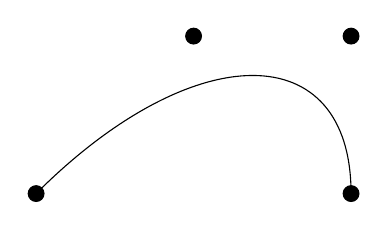
\begin{tikzpicture}
\draw (0,0) .. controls (2,2) 
    and (4,2) .. (4,0);
\filldraw (0,0) circle (.1)
    (2,2) circle (.1)
    (4,2) circle (.1)
    (4,0) circle (.1);
\end{tikzpicture}
}
\draw (0,0) .. controls (2,2) 
    and (4,2) .. (4,0);
\end{fdemo}

抛物线命令如下,除了起止点还可以指定顶点。
\begin{fdemo}{
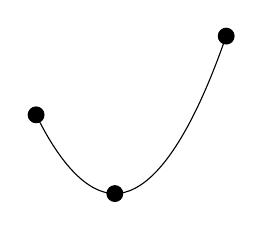
\begin{tikzpicture}
\draw (-1,1) parabola bend (0,0) (1.414,2);
\filldraw (-1,1) circle (.1)
    (0,0) circle (.1)
    (1.414,2) circle (.1);
\end{tikzpicture}
}
\draw (-1,1) parabola 
    bend (0,0) (1.414,2);
\end{fdemo}

\subsection{图形控制}
\subsubsection{线型和箭头}
绘图命令可以设置线型和箭头参数。
\begin{fdemo}{
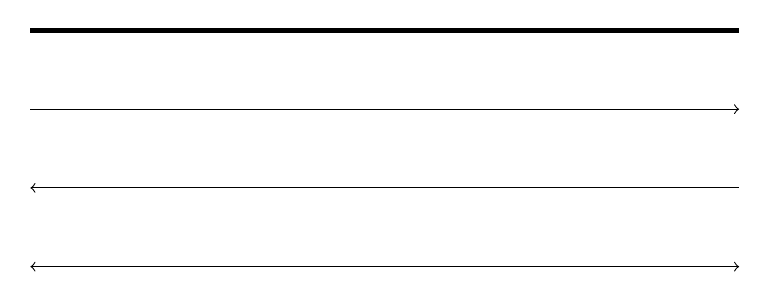
\begin{tikzpicture}
\draw[line width=2pt] (0,3)--(9,3);
\draw[->] (0,2)--(9,2);
\draw[<-] (0,1)--(9,1);
\draw[<->] (0,0)--(9,0);
\end{tikzpicture}
}
\draw[line width=2pt] (0,0)--(9,0);
\draw[->] (0,1)--(9,1);
\draw[<-] (0,2)--(9,2);
\draw[<->] (0,3)--(9,3);
\end{fdemo}

\subsubsection{颜色、填充、阴影}
颜色参数的用法如下。PGF~可以使用~\verb|xcolor|~宏包\citep{Kern_2007}中定义的所有颜色。
\begin{fdemo}{
\begin{tikzpicture}
\draw[red] (0,4)--(9,4);
\draw[green] (0,2)--(9,2);
\draw[blue] (0,0)--(9,0);
\end{tikzpicture}
}
\draw[red] (0,4)--(9,4);
\draw[green] (0,2)--(9,2);
\draw[blue] (0,0)--(9,0);
\end{fdemo}

封闭路径可以用颜色填充,\verb|\filldraw|~命令可以分别指定边框色和填充色。
\begin{fdemo}{
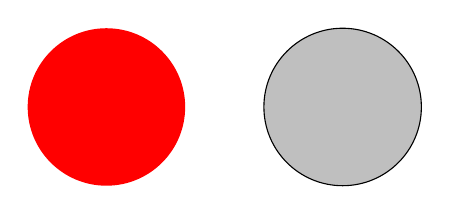
\begin{tikzpicture}
\fill[red] (1,1) circle (1);
\filldraw[fill=lightgray,draw=black] 
    (4,1) circle (1);
\end{tikzpicture}
}
\fill[red] (1,1) circle (1);
\filldraw[fill=lightgray,draw=black] 
    (4,1) circle (1);
\end{fdemo}

\verb|\shade|~命令可以产生渐变和光影效果,缺省是从上到下,灰色渐变为白色。我们也可以使用其它方向和颜色的渐变。
\begin{code}
\shade (0,0) rectangle (2,2);
\shade[left color=red,right color=orange] (3,0) rectangle (5,2);
\shade[inner color=red,outer color=orange] (6,0) rectangle (8,2);
\shade[ball color=blue] (10,1) circle (1);
\end{code}

\begin{out}

\begin{tikzpicture}
\shade (0,0) rectangle (2,2);
\shade[left color=red,right color=orange] (3,0) rectangle (5,2);
\shade[inner color=red,outer color=orange] (6,0) rectangle (8,2);
\shade[ball color=blue] (10,1) circle (1);
\end{tikzpicture}
\end{out}

\subsubsection{图形变换}
对图形对象可以进行平移和旋转操作,注意如果两种操作同时进行,它们是有顺序的。注意预定义的长度单位在这里对平移参数失效。
\begin{code}
\draw (0,0) rectangle (2,2);
\draw[xshift=30pt] (0,0) rectangle (2,2);
\draw[xshift=75pt,rotate=45] (0,0) rectangle (2,2);
\end{code}

\begin{out}
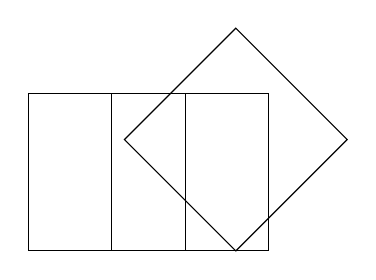
\begin{tikzpicture}
\draw (0,0) rectangle (2,2);
\draw[xshift=30pt] (0,0) rectangle (2,2);
\draw[xshift=75pt,rotate=45] (0,0) rectangle (2,2);
\end{tikzpicture}
\end{out}

\subsection{样式}
PGF~比~\MP~和~PSTricks~多了一个有趣的概念:样式(style),它的思路和~HTML~的~CSS~相近。我们可以先定义两种样式,
\tikzset{
    myline/.style={line width=2pt},
    myblueline/.style={myline,blue}
}
\begin{code}
\tikzset{
    myline/.style={line width=2pt},
    myblueline/.style={myline,blue}
}
\end{code}

然后就可以在绘图命令中这样使用样式。
\begin{fdemo}{
\begin{tikzpicture}
\draw[myline] (0,2)--(9,2);
\draw[myblueline] (0,0)--(9,0);
\end{tikzpicture}
}
\draw[myline] (0,2)--(9,2);
\draw[myblueline] (0,0)--(9,0);
\end{fdemo}

除了用~\verb|\tikzset|~命令定义样式,我们也可以在~\verb|tikzpicture|~环境头部声明样式。前者是全局性的,后者则是局部性的。
\begin{code}
\begin{tikzpicture}[
    thickline/.style=2pt,
    bluethickline/.style={thickline,color=blue}
]
...
\end{tikzpicture}
\end{code}

注意在样式中预定义长度单位有时会失效,所以最好使用绝对单位。

\subsection{流程图}
\subsubsection{节点}
PGF~中的节点(node)可以是简单的标签,也可以有各种形状的边框,还可以有各种复杂的属性。比如下例中的节点样式:\verb|box|,它的边框是矩形,有圆角;它有最小宽度、高度、文字和边框的距离,边框和填充颜色等属性。

\begin{code}
\tikzset{
    box/.style={rectangle, rounded corners=6pt, 
        minimum width=50pt, minimum height=20pt, inner sep=6pt, 
        draw=gray,thick, fill=lightgray}
}
\end{code}

除了上述类别属性,节点还可以有名字、位置等属性。在下例中,我们先画了三个有名字的文本框;然后用箭头把文本框连接起来,注意连接时要引用文本框的名字;接着在箭头上加了标签。
\begin{code}
\node[box] (tex) at(0,0) {.tex};  %文本框
\node[box] (dvi) at(10,0) {.dvi}; %文本框
\node[box] (pdf) at(20,0) {.pdf}; %文本框
\draw[->] (tex)--(dvi);           %箭头
\draw[->] (dvi)--(pdf);           %箭头
\node at (5,1) {latex};           %标签
\node at (15,1) {dvipdfmx};       %标签
\end{code}

\begin{out}
\begin{tikzpicture}
\node[box] (tex) at(0,0) {.tex};
\node[box] (dvi) at(10,0) {.dvi};
\node[box] (pdf) at(20,0) {.pdf};
\draw[->] (tex)--(dvi);
\draw[->] (dvi)--(pdf);
\node at (5,1) {latex};
\node at (15,1) {dvipdfmx};
\end{tikzpicture}
\end{out}

在上例中的节点都使用了绝对位置,PGF~中还可以使用更灵活一点的相对位置。比如在下例中,dvi~节点在~tex~节点右边~50pt~处(我们前面定义的基本长度单位是~10pt),而~pdf~节点又在~dvi~节点右边~50pt~处。

箭头可以换为专门用来连接节点的~\verb|edge|~;标签也改成相对位置,箭头上方~5pt~处。
\begin{code}
\node[box] (tex) {.tex};
\node[box,right=5 of tex] (dvi) {.dvi};
\node[box,right=6 of dvi] (pdf) {.pdf};
\path (tex) edge[->]  node[above=.5] {latex} (dvi)
    (dvi) edge[->] node[above=.5] {dvipdfmx} (pdf);
\end{code}

\begin{out}
\begin{tikzpicture}
\node[box] (tex) {.tex};
\node[box,right=5 of tex] (dvi) {.dvi};
\node[box,right=6 of dvi] (pdf) {.pdf};
\path (tex) edge[->]  node[above=.5] {latex} (dvi)
    (dvi) edge[->] node[above=.5] {dvipdfmx} (pdf);
\end{tikzpicture}
\end{out}

\subsubsection{树}
下面是一棵简单的树。我们可以用一个参数控制相邻节点的距离,预定义长度单位对此参数也会失效。
\begin{code}
\begin{tikzpicture}[sibling distance=80pt]
\node[box] {TeX}
    child {node[box] {Plain\TeX}}
    child {node[box] {\LaTeX}
        child {node[box] {MiKTeX}}
        child {node[box] {TeX Live}}
        child {node[box] {MacTeX}}
    };
\end{tikzpicture}
\end{code}

\begin{out}
\begin{tikzpicture}[sibling distance=80pt]
\node[box] {TeX}
    child {node[box] {Plain\TeX}}
    child {node[box] {\LaTeX}
        child {node[box] {MiKTeX}}
        child {node[box] {TeX Live}}
        child {node[box] {MacTeX}}
    };
\end{tikzpicture}
\end{out}

\bibliographystyle{unsrtnat}
\bibliography{reading}
\newpage
